% Choose one to switch between slides and handout
\documentclass[]{beamer}
%\documentclass[handout]{beamer}

% Video Meta Data
\title{Bitcoin, Blockchain and Cryptoassets}
\subtitle{Transaction Examples}
\author{Prof. Dr. Fabian Schär}
\institute{University of Basel}

% Config File
% Packages
\usepackage[utf8]{inputenc}
\usepackage{hyperref}
\usepackage{gitinfo2}
\usepackage{tikz}
\usepackage{amsmath}
\usepackage{mathtools}
\usepackage{bibentry}
\usepackage{xcolor}
\usepackage{colortbl} % Add colour to LaTeX tables
\usepackage{caption}
\usepackage[export]{adjustbox}
\usepackage{pgfplots} \pgfplotsset{compat = 1.17}
\usepackage{makecell}
\usepackage{fancybox}
\usepackage{ragged2e}
\usepackage{fontawesome}
\usepackage{seqsplit}
\usepackage{tabularx}

% Color Options
\definecolor{highlight}{rgb}{0.65,0.84,0.82}
\definecolor{focus}{rgb}{0.72, 0, 0}
\definecolor{lightred}{rgb}{0.8,0.5,0.5}
\definecolor{midgray}{RGB}{190,195,200}

% Beamer Template Options
\beamertemplatenavigationsymbolsempty
\setbeamertemplate{footline}[frame number]
\setbeamercolor{structure}{fg=black}
\setbeamercolor{footline}{fg=black}
\setbeamercolor{title}{fg=black}
\setbeamercolor{frametitle}{fg=black}
\setbeamercolor{item}{fg=black}
\setbeamercolor{}{fg=black}
\setbeamercolor{bibliography item}{fg=black}
\setbeamercolor*{bibliography entry title}{fg=black}
\setbeamercolor{alerted text}{fg=focus}
\setbeamertemplate{items}[square]
\setbeamertemplate{enumerate items}[default]
\captionsetup[figure]{labelfont={color=black},font={color=black}}
\captionsetup[table]{labelfont={color=black},font={color=black}}

\setbeamertemplate{bibliography item}{\insertbiblabel}

% Link Icon Command
\newcommand{\link}{%
    \tikz[x=1.2ex, y=1.2ex, baseline=-0.05ex]{%
        \begin{scope}[x=1ex, y=1ex]
            \clip (-0.1,-0.1)
                --++ (-0, 1.2)
                --++ (0.6, 0)
                --++ (0, -0.6)
                --++ (0.6, 0)
                --++ (0, -1);
            \path[draw,
                line width = 0.5,
                rounded corners=0.5]
                (0,0) rectangle (1,1);
        \end{scope}
        \path[draw, line width = 0.5] (0.5, 0.5)
            -- (1, 1);
        \path[draw, line width = 0.5] (0.6, 1)
            -- (1, 1) -- (1, 0.6);
        }
    }

% Read Git Data from Github Actions Workflow
% Defaults to gitinfo2 for local builds
\IfFileExists{gitInfo.txt}
	{\input{gitInfo.txt}}
	{
		\newcommand{\gitRelease}{(Local Release)}
		\newcommand{\gitSHA}{\gitHash}
		\newcommand{\gitDate}{\gitAuthorIsoDate}
	}

% Custom Titlepage
\defbeamertemplate*{title page}{customized}[1][]
{
  \vspace{-0cm}\hfill\includegraphics[width=2.5cm]{../config/logo_cif}
  \includegraphics[width=1.9cm]{../config/seal_wwz}
  \\ \vspace{2em}
  \usebeamerfont{title}\textbf{\inserttitle}\par
  \usebeamerfont{title}\usebeamercolor[fg]{title}\insertsubtitle\par  \vspace{1.5em}
  \small\usebeamerfont{author}\insertauthor\par
  \usebeamerfont{author}\insertinstitute\par \vspace{2em}
  \usebeamercolor[fg]{titlegraphic}\inserttitlegraphic
    \tiny \noindent \texttt{Release Ver.: \gitRelease}\\ 
    \texttt{Version Hash: \gitSHA}\\
    \texttt{Version Date: \gitDate}\\ \vspace{1em}
    
    
    \iffalse
  \link \href{https://github.com/cifunibas/Bitcoin-Blockchain-Cryptoassets/blob/main/slides/intro.pdf}
  {Get most recent version}\\
  \link \href{https://github.com/cifunibas/Bitcoin-Blockchain-Cryptoassets/blob/main/slides/intro.pdf}
  {Watch video lecture}\\ 
  
  \fi
  
  \vspace{1em}
  License: \texttt{Creative Commons Attribution-NonCommercial-ShareAlike 4.0 International}\\\vspace{2em}
  \includegraphics[width = 1.2cm]{../config/license}
}


% tikzlibraries
\usetikzlibrary{decorations.pathreplacing}
\usetikzlibrary{decorations.markings}
\usetikzlibrary{positioning}
\usetikzlibrary{calc}
\captionsetup{font=footnotesize}

\usepackage{fancybox}

%%%%%%%%%%%%%%%%%%%%%%%%%%%%%%%%%%%%%%%%%%%%%%
%%%%%%%%%%%%%%%%%%%%%%%%%%%%%%%%%%%%%%%%%%%%%%
\begin{document}

\thispagestyle{empty}
\begin{frame}[noframenumbering]
	\titlepage
\end{frame}

%%%
%\begin{frame}{Prerequisites: Hexadecimal}
%Hexadecimal (Base 16)
%\vspace{1em}
%\begin{itemize}
%	\item Numbers 1-9, Letters a-f
%	\item Two hexadecimal values make up one byte ($16^{2} = 2^{8}$)
%\end{itemize}
%\end{frame}
%%%


%%%
\begin{frame}{Prerequisites}
\begin{itemize}
	\item<1->{Hexadecimal values (Base 16)}
	\item<2->{Endianness:}
		\begin{itemize}
			\item<2->{1 in big-endian: 00000001}
			\item<3->{1 in little-endian: 01000000}
		\end{itemize}
	\item<4->{Hash functions}
	\item<5->{ECDSA}\\
\end{itemize}

%Refers to the memory organisation for simple numerical values, primarily the storage of integers in the working memory.
%\vspace{1em}
%\begin{itemize}
%	\item Big-endian: Most significant byte is stored first, i.e. at the smallest memory address.
%	\item 1 in big-endian: 00000001
%	\item Little-endian: Least significant byte is stored at the starting address.
%	\item 1 in little-endian: 01000000
%\end{itemize}
\end{frame}
%%%	


%%%
\begin{frame}{Pay-to-Public-Key}
	\href{https://blockstream.info/tx/f4184fc596403b9d638783cf57adfe4c75c605f6356fbc91338530e9831e9e16}{\link The first Bitcoin transaction:}
	\begin{figure}
		\begin{tikzpicture}
	\node (Satoshi) at (-3,0)[label=below: Satoshi Nakamoto] {
\includegraphics[height = 0.2\textheight]{../assets/images/agents/handing_money_right.png}};
	\node (Hal) at (3, 0)[label=below: Hal Finney] {
\includegraphics[height = 0.2\textheight]{../assets/images/agents/reaching_left.png}};
	
	\uncover<2->{
		\draw[->, ultra thick] (Satoshi.east) -- (Hal.west) node[midway, above] {10 BTC};
	}
	
	\uncover<3->{
		\node (pubKey1) at (-3, -3.5) {\scriptsize{$K_{pub}^{SN} = $
		\begin{tabular}{l} \texttt{04}\\
			\texttt{\color{focus}{11db93e1dcdb8a01}}\\
			\texttt{\color{focus}{6b49840f8c53bc1e}}\\
			\texttt{\color{focus}{b68a382e97b1482e}}\\
			\texttt{\color{focus}{cad7b148a6909a5c}}\\
			\texttt{\color{highlight}{b2e0eaddfb84ccf9}}\\
			\texttt{\color{highlight}{744464f82e160bfa}}\\
			\texttt{\color{highlight}{9b8b64f9d4c03f99}}\\
			\texttt{\color{highlight}{9b8643f656b412a3}}\\
		\end{tabular}}};
	}
	
	\uncover<3->{
		\node (pubKey1) at (3, -3.5) {\scriptsize{$K_{pub}^{HF} = $
		\begin{tabular}{l} \texttt{04}\\
			\texttt{\color{focus}{ae1a62fe09c5f51b}}\\
			\texttt{\color{focus}{13905f07f06b99a2}}\\
			\texttt{\color{focus}{f7159b2225f374cd}}\\
			\texttt{\color{focus}{378d71302fa28414}}\\
			\texttt{\color{highlight}{e7aab37397f554a7}}\\
			\texttt{\color{highlight}{df5f142c21c1b730}}\\
			\texttt{\color{highlight}{3b8a0626f1baded5}}\\
			\texttt{\color{highlight}{c72a704f7e6cd84c}}
		\end{tabular}}};
	}
	
\end{tikzpicture}
	\end{figure}
	
%\begin{itemize}
%\item Satoshi mined 50 BTC and has a plan \dots
%\item He wants to send 10 BTC to his friend Hal Finney.
%\item He does that by sending 10 BTC to Finney's Public Key.
%\item Since he has to reference the whole UTXO, he returns the remaining 40 BTC to himself.
%\item How does Satoshi form this transaction?
%\end{itemize}
\end{frame}
%%%

\begin{frame}{Transaction Inputs}
	\begin{figure}
		 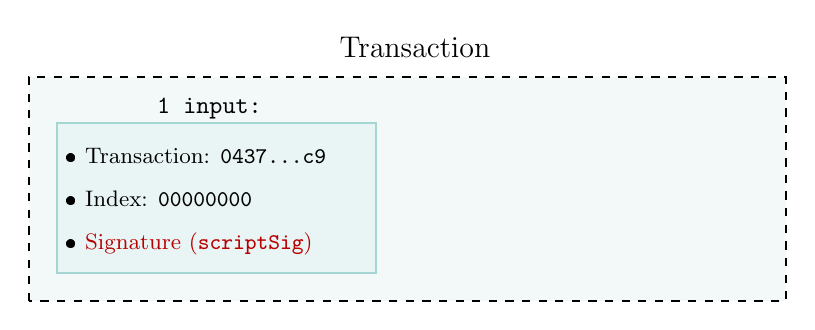
\begin{tikzpicture}[scale=0.9, every node/.style={scale=0.9}]
    
        \filldraw[yshift=-0.05cm, xshift=0.1cm,color = highlight!15, thick, draw=black, dashed] (-4,-4) rectangle ++(304pt,90pt) ;
    
        \filldraw[yshift=-0.05cm, xshift=0.1cm,color = highlight!25, thick, draw=highlight] (-3.6,-3.6) rectangle ++(128pt,60pt) ;
     
    \draw[color=black] plot (-1.35,-1.6) node[above] {\texttt{1 input:}};
    \draw[color=black] plot (-3.5,-2) node[right] {\small{\textbullet{} Transaction: \texttt{0437...c9}}};
    \draw[color=black] plot (-3.5,-2.6)   node[right] {\small{\textbullet{} Index: \texttt{00000000}}};
    \draw[color=black] plot (-3.5,-3.25)   node[right] {\small{\textbullet{} \textcolor{focus}{Signature (\texttt{scriptSig})}}};
    \draw[color=black] plot (1.55,-0.2) node [below]
    {\large{{Transaction}}};
    
\end{tikzpicture}
	\end{figure}
	\uncover<2->{
		\scriptsize
			\begin{tabular}{ll}
				\texttt{scriptPubKey} from the previous transaction: & \\
				\texttt{OP\_PUSHBYTES\_65:} & \texttt{41}\\
				Uncompressed public key: & \texttt{04}\\
				Public key: & \texttt{11db93e1dcdb8a016b49840f8c53bc1e}\\
				 & \texttt{b68a382e97b1482ecad7b148a6909a5c}\\
				 & \texttt{b2e0eaddfb84ccf9744464f82e160bfa}\\
				 & \texttt{9b8b64f9d4c03f999b8643f656b412a3}\\
				\texttt{OP\_CHECKSIG:} & \texttt{ac}
			\end{tabular}
	}
	\vspace{0.5em}\\
	\small
	\uncover<3->{$\rightarrow$ If you know the private key to \texttt{11db...a3} you can spend the UTXO \phantom{$\rightarrow$} of 50 BTC.}
\end{frame}

\begin{frame}{Transaction Outputs}
	\begin{figure}
		 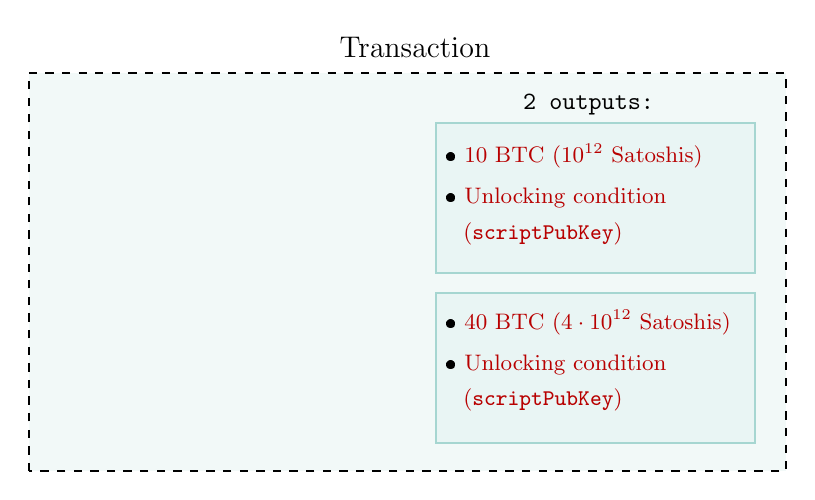
\begin{tikzpicture}[scale=0.9, every node/.style={scale=0.9}]
    
        \filldraw[yshift=-0.05cm, xshift=0.1cm,color = highlight!15, thick, draw=black, dashed] (-4,-6.4) rectangle ++(304pt,160pt) ;
        
    \draw[color=black] plot (1.55,-0.2) node [below]
    {\large{{Transaction}}};

    
        \filldraw[yshift=-0.05cm, xshift=0.1cm,color = highlight!25, thick, draw=highlight] (1.75,-3.6) rectangle ++(128pt,60pt) ;
    
    \draw[color=black] plot (4,-1.55)   node[above] {\texttt{2 outputs:}};
    \draw[color=black] plot (1.85,-2)   node[right] {\small{\textbullet{} \textcolor{focus}{10 BTC ($10^{12}$ Satoshis)}}};
    \draw[color=black] plot (1.85,-2.6)   node[right] {\small{\textbullet{} \textcolor{focus}{Unlocking condition}}};
    \draw[color=black] plot (2,-3.1)   node[right] {\small{ \textcolor{focus}{(\texttt{scriptPubKey})}}};

	\filldraw[yshift=-0.05cm, xshift=0.1cm,color = highlight!25, thick, draw=highlight] (1.75,-6) rectangle ++(128pt,60pt) ;

    \draw[color=black] plot (1.85,-4.35)   node[right] {\small{\textbullet{} \textcolor{focus}{40 BTC ($4 \cdot 10^{12}$ Satoshis)}}};
    \draw[color=black] plot (1.85,-4.95)   node[right] {\small{\textbullet{} \textcolor{focus}{Unlocking condition}}};
    \draw[color=black] plot (2,-5.45)   node[right] {\small{ \textcolor{focus}{(\texttt{scriptPubKey})}}};

\end{tikzpicture}
	\end{figure}
\end{frame}

\begin{frame}{Transaction Outputs}
	\scriptsize
	\textbf{First output:}\\
	\begin{tabular}{ll}
	10 BTC & = 1,000,000,000 Satoshis\\
	\uncover<2->{& = \texttt{00ca9a3b00000000} as little-endian integer}\\
	\uncover<3->{\texttt{scriptPubKey:} & \\
		\texttt{OP\_PUSHBYTES\_65:} & \texttt{41}\\
		Uncompressed public key: & \texttt{04}\\
		Public key: & \texttt{ae1a62fe09c5f51b13905f07f06b99a2}\\
		 & \texttt{f7159b2225f374cd378d71302fa28414}\\
		 & \texttt{e7aab37397f554a7df5f142c21c1b730}\\
		 & \texttt{3b8a0626f1baded5c72a704f7e6cd84c}\\
		\texttt{OP\_CHECKSIG:} & \texttt{ac}
	}
	\end{tabular}
	\vspace{1em}\\
	\textbf{Second output (''change"):}\\
	\begin{tabular}{ll}
	40 BTC & = 4,000,000,000 Satoshis\\
	\uncover<2->{& = \texttt{00286bee00000000} as little-endian integer}\\
	\uncover<3->{\texttt{scriptPubKey:} & \\
		\texttt{OP\_PUSHBYTES\_65:} & \texttt{41}\\
		Uncompressed public key: & \texttt{04}\\
		Public key: & \texttt{11db93e1dcdb8a016b49840f8c53bc1e}\\
		 & \texttt{b68a382e97b1482ecad7b148a6909a5c}\\
		 & \texttt{b2e0eaddfb84ccf9744464f82e160bfa}\\
		 & \texttt{9b8b64f9d4c03f999b8643f656b412a3}\\
		\texttt{OP\_CHECKSIG:} & \texttt{ac}
	}
	\end{tabular}

\end{frame}

\begin{frame}{Transaction Inputs and Outputs}
	\begin{figure}
		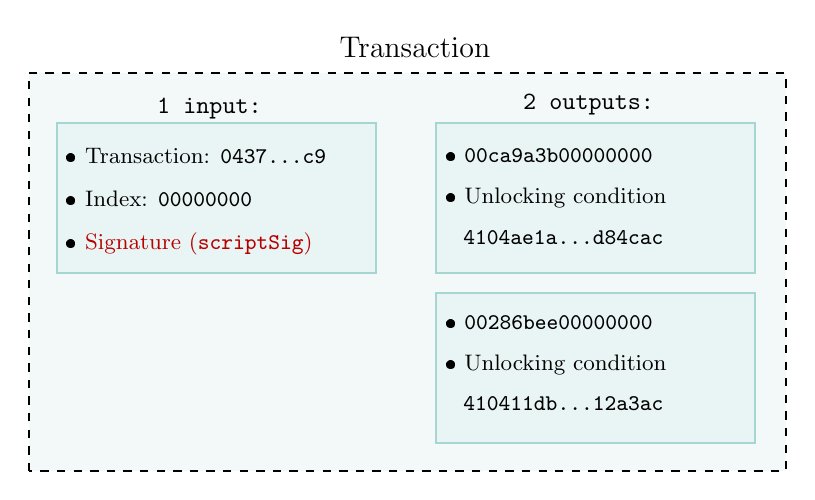
\begin{tikzpicture}[scale=0.9, every node/.style={scale=0.9}]
    
        \filldraw[yshift=-0.05cm, xshift=0.1cm,color = highlight!15, thick, draw=black, dashed] (-4,-6.4) rectangle ++(304pt,160pt) ;
        
    \draw[color=black] plot (1.55,-0.2) node [below]
    {\large{{Transaction}}};

    
    \filldraw[yshift=-0.05cm, xshift=0.1cm,color = highlight!25, thick, draw=highlight] (1.75,-3.6) rectangle ++(128pt,60pt) ;
    
    \filldraw[yshift=-0.05cm, xshift=0.1cm,color = highlight!25, thick, draw=highlight] (-3.6,-3.6) rectangle ++(128pt,60pt) ;
     
    \draw[color=black] plot (-1.35,-1.6) node[above] {\texttt{1 input:}};
    \draw[color=black] plot (-3.5,-2) node[right] {\small{\textbullet{} Transaction: \texttt{0437...c9}}};
    \draw[color=black] plot (-3.5,-2.6)   node[right] {\small{\textbullet{} Index: \texttt{00000000}}};
    \draw[color=black] plot (-3.5,-3.25)   node[right] {\small{\textbullet{} \textcolor{focus}{Signature (\texttt{scriptSig})}}};

    
    \draw[color=black] plot (4,-1.55)   node[above] {\texttt{2 outputs:}};
    \draw[color=black] plot (1.85,-2)   node[right] {\small{\textbullet{} \texttt{00ca9a3b00000000}}};
    \draw[color=black] plot (1.85,-2.6)   node[right] {\small{\textbullet{} Unlocking condition}};
    \draw[color=black] plot (2,-3.15)   node[right] {\small{ \texttt{4104ae1a...d84cac}}};

	\filldraw[yshift=-0.05cm, xshift=0.1cm,color = highlight!25, thick, draw=highlight] (1.75,-6) rectangle ++(128pt,60pt) ;

    \draw[color=black] plot (1.85,-4.35)   node[right] {\small{\textbullet{} \texttt{00286bee00000000}}};
    \draw[color=black] plot (1.85,-4.95)   node[right] {\small{\textbullet{} Unlocking condition}};
    \draw[color=black] plot (2,-5.5)   node[right] {\small{ \texttt{410411db...12a3ac}}};

\end{tikzpicture}	
	\end{figure}

\end{frame}


%%%
%\begin{frame}{Transaction Hash}
%\begin{itemize}
%\item Transaction Hash: \\
%{\scriptsize \texttt{f4184fc596403b9d638783cf57adfe4c75c605f6356fbc91338530e9831e9e16}}
%\item SHA256(SHA256(Raw TRX Data)) $\rightarrow$ TRX Hash
%\end{itemize}
%\end{frame}
%%%	


%%%
\begin{frame}{Raw Transaction Data}
\begin{scriptsize}
\texttt{01000000\textcolor{highlight}{01c997a5e56e104102fa209c6a852dd90660a20b2d9c352423edce25857fcd3704
00000000}\textcolor{focus}{4847304402204e45e16932b8af514961a1d3a1a25fdf3f4f7732e9d624c6c61548
ab5fb8cd410220181522ec8eca07de4860a4acdd12909d831cc56cbbac4622082221a8768d
1d0901}ffffffff\textcolor{highlight}{0200ca9a3b00000000434104ae1a62fe09c5f51b13905f07f06b99a2f715
9b2225f374cd378d71302fa28414e7aab37397f554a7df5f142c21c1b7303b8a0626f1bade
d5c72a704f7e6cd84cac00286bee0000000043410411db93e1dcdb8a016b49840f8c53bc1e
b68a382e97b1482ecad7b148a6909a5cb2e0eaddfb84ccf9744464f82e160bfa9b8b64f9d4
c03f999b8643f656b412a3ac}00000000}
\end{scriptsize}
\scriptsize
\begin{itemize}
	\item<2-> Version as little-endian integer: \texttt{01000000}
	\item<2-> Sequence number (deprecated): \texttt{ffffffff}
	\item<2-> Timelock: \texttt{00000000}
\end{itemize}
\end{frame}
%%%

%%%
\begin{frame}{Raw Transaction Data (Input)}
\begin{scriptsize}
\texttt{01000000\textcolor{highlight}{01c997a5e56e104102fa209c6a852dd90660a20b2d9c352423edce25857fcd3704
00000000}\textcolor{focus}{4847304402204e45e16932b8af514961a1d3a1a25fdf3f4f7732e9d624c6c61548
ab5fb8cd410220181522ec8eca07de4860a4acdd12909d831cc56cbbac4622082221a8768d
1d0901}ffffffff\textcolor{highlight}{0200ca9a3b00000000434104ae1a62fe09c5f51b13905f07f06b99a2f715
9b2225f374cd378d71302fa28414e7aab37397f554a7df5f142c21c1b7303b8a0626f1bade
d5c72a704f7e6cd84cac00286bee0000000043410411db93e1dcdb8a016b49840f8c53bc1e
b68a382e97b1482ecad7b148a6909a5cb2e0eaddfb84ccf9744464f82e160bfa9b8b64f9d4
c03f999b8643f656b412a3ac}00000000}
\end{scriptsize}
\scriptsize
\begin{itemize}
	\item 1 input: \texttt{01}
	\item Previous transaction in reverse byte order: \texttt{c997a5e56e104102fa209c6a852dd90660a20b2d9c352423edce25857fcd3704}
	\item Index of the output within the previous transaction as little-endian integer: \texttt{00000000}
\end{itemize}
\end{frame}
%%%


%%%
\begin{frame}{Raw Transaction Data (Outputs)}
\begin{scriptsize}
\texttt{01000000\textcolor{highlight}{01c997a5e56e104102fa209c6a852dd90660a20b2d9c352423edce25857fcd3704
00000000}\textcolor{focus}{4847304402204e45e16932b8af514961a1d3a1a25fdf3f4f7732e9d624c6c61548
ab5fb8cd410220181522ec8eca07de4860a4acdd12909d831cc56cbbac4622082221a8768d
1d0901}ffffffff\textcolor{highlight}{0200ca9a3b00000000434104ae1a62fe09c5f51b13905f07f06b99a2f715
9b2225f374cd378d71302fa28414e7aab37397f554a7df5f142c21c1b7303b8a0626f1bade
d5c72a704f7e6cd84cac00286bee0000000043410411db93e1dcdb8a016b49840f8c53bc1e
b68a382e97b1482ecad7b148a6909a5cb2e0eaddfb84ccf9744464f82e160bfa9b8b64f9d4
c03f999b8643f656b412a3ac}00000000}
\end{scriptsize}
\scriptsize
\begin{itemize}
	\item 2 outputs: \texttt{02}
	\item 10 BTC: \texttt{00ca9a3b00000000}
	\item 67 byte long \texttt{scriptPubKey}: \texttt{43}
	\item 65 byte long uncompressed public key: \texttt{4104}
	\item Public key
	\item \texttt{OP\_CHECKSIG}: \texttt{ac}
	\item 40 BTC ''change": \texttt{00286bee00000000}
	\item 67 byte long \texttt{scriptPubKey}: \texttt{43}
	\item 65 byte long uncompressed public key: \texttt{4104}
	\item Public key
	\item \texttt{OP\_CHECKSIG}: \texttt{ac}
\end{itemize}
\end{frame}
%%%

%%%
\begin{frame}{Raw Transaction Data (Signature)}
	\begin{scriptsize}
\texttt{01000000\textcolor{highlight}{01c997a5e56e104102fa209c6a852dd90660a20b2d9c352423edce25857fcd3704
00000000}\textcolor{focus}{4847304402204e45e16932b8af514961a1d3a1a25fdf3f4f7732e9d624c6c61548
ab5fb8cd410220181522ec8eca07de4860a4acdd12909d831cc56cbbac4622082221a8768d
1d0901}ffffffff\textcolor{highlight}{0200ca9a3b00000000434104ae1a62fe09c5f51b13905f07f06b99a2f715
9b2225f374cd378d71302fa28414e7aab37397f554a7df5f142c21c1b7303b8a0626f1bade
d5c72a704f7e6cd84cac00286bee0000000043410411db93e1dcdb8a016b49840f8c53bc1e
b68a382e97b1482ecad7b148a6909a5cb2e0eaddfb84ccf9744464f82e160bfa9b8b64f9d4
c03f999b8643f656b412a3ac}00000000}
\end{scriptsize}
\scriptsize
\begin{itemize}
	\item 72 byte long \texttt{scriptSig}: \texttt{48}
	\item 71 byte long signature: \texttt{47}
	\item DER sequence follows: \texttt{30}
	\item 68 bytes long: \texttt{44}
	\item An integer follows: \texttt{02}
	\item The integer is 32 bytes long: \texttt{20}
	\item $r$ from the ECDSA signature: \texttt{4e45e16932b8af514961a1d3a1a25fdf3f4f7732e9d624c6c61548ab5fb8cd41}
	\item An integer follows: \texttt{02}
	\item The integer is 32 bytes long: \texttt{20}
	\item $s$ from the ECDSA signature: \texttt{181522ec8eca07de4860a4acdd12909d831cc56cbbac4622082221a8768d1d09}
	\item \texttt{SIGHASH\_ALL}: \texttt{01}
\end{itemize}
\end{frame}
%%%

%%%
\begin{frame}{Signature}
	We do not know Satoshi's private key.\\
	What is signed exactly? Transaction message?	\\
	How is it encoded?
\end{frame}
%%%

%%%
\begin{frame}{Verification}
	Script:\\
	Define Bitcoin's elliptic curve and the generator point.\\
	Define Satoshi's public key.\\
	Get $r$ and $s$ from the \texttt{scriptSig}.\\
	We know the transaction message from the last slide.\\
	Find $u_1$ and $u_2$.\\
	Find $P$.\\
	Authentic if $P_x\ (mod\ p) == r$ is true.\\
\end{frame}
%%%

%%%%
%\begin{frame}[t]{Version}
%\shadowbox{
%\begin{minipage}[c]{4.2in}
%\begin{tiny}
%\texttt{\textcolor{focus}{01000000}\textcolor{black!30}{01c997a5e56e104102fa209c6a852dd90660a20b2d9c352423edce25857fcd3704000000004847304402204e
%45e16932b8af514961a1d3a1a25fdf3f4f7732e9d624c6c61548ab5fb8cd410220181522ec8eca07de4860a4acdd1290
%9d831cc56cbbac4622082221a8768d1d0901ffffffff0200ca9a3b00000000434104ae1a62fe09c5f51b13905f07f06b
%99a2f7159b2225f374cd378d71302fa28414e7aab37397f554a7df5f142c21c1b7303b8a0626f1baded5c72a704f7e6c
%d84cac00286bee0000000043410411db93e1dcdb8a016b49840f8c53bc1eb68a382e97b1482ecad7b148a6909a5cb2e0
%eaddfb84ccf9744464f82e160bfa9b8b64f9d4c03f999b8643f656b412a3ac00000000}}
%\end{tiny}
%\end{minipage}
%}
%\begin{itemize}
%	\item Version as a little-endian integer: \textcolor{focus}{01000000}
%\end{itemize}
%\end{frame}
%%%%
%
%
%%%%
%\begin{frame}[t]{Transaction Inputs}
%\shadowbox{
%\begin{minipage}[c]{4.2in}
%\begin{tiny}
%\texttt{\textcolor{black!30}{01000000}\textcolor{black}{01c997a5e56e104102fa209c6a852dd90660a20b2d9c352423edce25857fcd3704000000004847304402204e
%45e16932b8af514961a1d3a1a25fdf3f4f7732e9d624c6c61548ab5fb8cd410220181522ec8eca07de4860a4acdd1290
%9d831cc56cbbac4622082221a8768d1d0901ffffffff}\textcolor{black!30}{0200ca9a3b00000000434104ae1a62fe09c5f51b13905f07f06b
%99a2f7159b2225f374cd378d71302fa28414e7aab37397f554a7df5f142c21c1b7303b8a0626f1baded5c72a704f7e6c
%d84cac00286bee0000000043410411db93e1dcdb8a016b49840f8c53bc1eb68a382e97b1482ecad7b148a6909a5cb2e0
%eaddfb84ccf9744464f82e160bfa9b8b64f9d4c03f999b8643f656b412a3ac00000000}}
%\end{tiny}
%\end{minipage}
%}
%\begin{itemize}
%	\item Raw Transaction Input Data
%\end{itemize}
%\end{frame}
%%%%
%
%
%%%%
%\begin{frame}[t]{Number of Inputs}
%\shadowbox{
%\begin{minipage}[c]{4.2in}
%\begin{tiny}
%\texttt{\textcolor{black!30}{01000000}\textcolor{black!60}{\textcolor{focus}{01}c997a5e56e104102fa209c6a852dd90660a20b2d9c352423edce25857fcd3704000000004847304402204e
%45e16932b8af514961a1d3a1a25fdf3f4f7732e9d624c6c61548ab5fb8cd410220181522ec8eca07de4860a4acdd1290
%9d831cc56cbbac4622082221a8768d1d0901ffffffff}\textcolor{black!30}{0200ca9a3b00000000434104ae1a62fe09c5f51b13905f07f06b
%99a2f7159b2225f374cd378d71302fa28414e7aab37397f554a7df5f142c21c1b7303b8a0626f1baded5c72a704f7e6c
%d84cac00286bee0000000043410411db93e1dcdb8a016b49840f8c53bc1eb68a382e97b1482ecad7b148a6909a5cb2e0
%eaddfb84ccf9744464f82e160bfa9b8b64f9d4c03f999b8643f656b412a3ac00000000}}
%\end{tiny}
%\end{minipage}
%}
%\begin{itemize}
%	\item Number of Inputs: \textcolor{focus}{01}
%\end{itemize}
%\end{frame}
%%%%
%
%
%%%%
%\begin{frame}[t]{Reference to previous transaction}
%\shadowbox{
%\begin{minipage}[c]{4.2in}
%\begin{tiny}
%\texttt{\textcolor{black!30}{01000000}\textcolor{black!60}{01\textcolor{focus}{c997a5e56e104102fa209c6a852dd90660a20b2d9c352423edce25857fcd3704}000000004847304402204e
%45e16932b8af514961a1d3a1a25fdf3f4f7732e9d624c6c61548ab5fb8cd410220181522ec8eca07de4860a4acdd1290
%9d831cc56cbbac4622082221a8768d1d0901ffffffff}\textcolor{black!30}{0200ca9a3b00000000434104ae1a62fe09c5f51b13905f07f06b
%99a2f7159b2225f374cd378d71302fa28414e7aab37397f554a7df5f142c21c1b7303b8a0626f1baded5c72a704f7e6c
%d84cac00286bee0000000043410411db93e1dcdb8a016b49840f8c53bc1eb68a382e97b1482ecad7b148a6909a5cb2e0
%eaddfb84ccf9744464f82e160bfa9b8b64f9d4c03f999b8643f656b412a3ac00000000}}
%\end{tiny}
%\end{minipage}
%}
%\begin{itemize}
%	\item Reverse byte order of previous transaction: \\ {\scriptsize
%	{c997a5e56e104102fa209c6a852dd90660a20b2d9c352423edce25857fcd3704}}
%	\item Coinbase transaction in Block 9.
%\end{itemize}
%\end{frame}
%%%%
%
%
%%%%
%\begin{frame}[t]{Inputs}
%\shadowbox{
%\begin{minipage}[c]{4.2in}
%\begin{tiny}
%\texttt{\textcolor{black!30}{01000000}\textcolor{black!60}{01c997a5e56e104102fa209c6a852dd90660a20b2d9c352423edce25857fcd3704\textcolor{focus}{00000000}4847304402204e
%45e16932b8af514961a1d3a1a25fdf3f4f7732e9d624c6c61548ab5fb8cd410220181522ec8eca07de4860a4acdd1290
%9d831cc56cbbac4622082221a8768d1d0901ffffffff}\textcolor{black!30}{0200ca9a3b00000000434104ae1a62fe09c5f51b13905f07f06b
%99a2f7159b2225f374cd378d71302fa28414e7aab37397f554a7df5f142c21c1b7303b8a0626f1baded5c72a704f7e6c
%d84cac00286bee0000000043410411db93e1dcdb8a016b49840f8c53bc1eb68a382e97b1482ecad7b148a6909a5cb2e0
%eaddfb84ccf9744464f82e160bfa9b8b64f9d4c03f999b8643f656b412a3ac00000000}}
%\end{tiny}
%\end{minipage}
%}
%\begin{itemize}
%	\item Index of Output within previous transaction as little-endian integer: \textcolor{focus}{00000000}
%\end{itemize}
%\end{frame}
%%%%
%
%
%%%%
%\begin{frame}[t]{Bytes length \texttt{scriptSig}}
%\shadowbox{
%\begin{minipage}[c]{4.2in}
%\begin{tiny}
%\texttt{\textcolor{black!30}{01000000}\textcolor{black!60}{01c997a5e56e104102fa209c6a852dd90660a20b2d9c352423edce25857fcd370400000000\textcolor{focus}{48}47304402204e
%45e16932b8af514961a1d3a1a25fdf3f4f7732e9d624c6c61548ab5fb8cd410220181522ec8eca07de4860a4acdd1290
%9d831cc56cbbac4622082221a8768d1d0901ffffffff}\textcolor{black!30}{0200ca9a3b00000000434104ae1a62fe09c5f51b13905f07f06b
%99a2f7159b2225f374cd378d71302fa28414e7aab37397f554a7df5f142c21c1b7303b8a0626f1baded5c72a704f7e6c
%d84cac00286bee0000000043410411db93e1dcdb8a016b49840f8c53bc1eb68a382e97b1482ecad7b148a6909a5cb2e0
%eaddfb84ccf9744464f82e160bfa9b8b64f9d4c03f999b8643f656b412a3ac00000000}}
%\end{tiny}
%\end{minipage}
%}
%\begin{itemize}
%	\item \textcolor{focus}{48} (72 in dec): Specifies bytes length of the following \texttt{scriptSig}.
%	\item In P2PK, \texttt{ScriptSig} only contains the signature, which is derived by the ECDSA of the private key.
%\end{itemize}
%\end{frame}
%%%%
%
%
%%%%
%\begin{frame}[t]{\texttt{scriptSig}}
%\shadowbox{
%\begin{minipage}[c]{4.2in}
%\begin{tiny}
%\texttt{\textcolor{black!30}{01000000}\textcolor{black!60}{01c997a5e56e104102fa209c6a852dd90660a20b2d9c352423edce25857fcd37040000000048\textcolor{focus}{47304402204e
%45e16932b8af514961a1d3a1a25fdf3f4f7732e9d624c6c61548ab5fb8cd410220181522ec8eca07de4860a4acdd1290
%9d831cc56cbbac4622082221a8768d1d0901}ffffffff}\textcolor{black!30}{0200ca9a3b00000000434104ae1a62fe09c5f51b13905f07f06b
%99a2f7159b2225f374cd378d71302fa28414e7aab37397f554a7df5f142c21c1b7303b8a0626f1baded5c72a704f7e6c
%d84cac00286bee0000000043410411db93e1dcdb8a016b49840f8c53bc1eb68a382e97b1482ecad7b148a6909a5cb2e0
%eaddfb84ccf9744464f82e160bfa9b8b64f9d4c03f999b8643f656b412a3ac00000000}}
%\end{tiny}
%\end{minipage}
%}
%\begin{itemize}
%	\item \textcolor{focus}{47} (71 in dec): Specifies bytes length of the following signature.
%	\item {\scriptsize\textcolor{focus}{30 44 02 20 4e 45 e1 69 32 b8 af 51 49 61 a1 d3 a1 a2 5f df 3f 4f 77 32 e9 d6 24 c6 c6 15 48 ab 5f b8 cd 41 02 20 18 15 22 ec 8e ca 07 de 48 60 a4 ac dd 12 90 9d 83 1c c5 6c bb ac 46 22 08 22 21 a8 76 8d 1d 09 01}}
%	\item Signature that matches Public Key defined in the \texttt{scriptPubKey} of the previous transaction.
%\end{itemize}
%\end{frame}
%%%%
%
%
%%%%
%\begin{frame}[t]{Sequence Number}
%\shadowbox{
%\begin{minipage}[c]{4.2in}
%\begin{tiny}
%\texttt{\textcolor{black!30}{01000000}\textcolor{black!60}{01c997a5e56e104102fa209c6a852dd90660a20b2d9c352423edce25857fcd3704000000004847304402204e
%45e16932b8af514961a1d3a1a25fdf3f4f7732e9d624c6c61548ab5fb8cd410220181522ec8eca07de4860a4acdd1290
%9d831cc56cbbac4622082221a8768d1d0901\textcolor{focus}{ffffffff}}\textcolor{black!30}{0200ca9a3b00000000434104ae1a62fe09c5f51b13905f07f06b
%99a2f7159b2225f374cd378d71302fa28414e7aab37397f554a7df5f142c21c1b7303b8a0626f1baded5c72a704f7e6c
%d84cac00286bee0000000043410411db93e1dcdb8a016b49840f8c53bc1eb68a382e97b1482ecad7b148a6909a5cb2e0
%eaddfb84ccf9744464f82e160bfa9b8b64f9d4c03f999b8643f656b412a3ac00000000}}
%\end{tiny}
%\end{minipage}
%}
%\begin{itemize}
%	\item \textcolor{focus}{ffffffff}
%	\item Default Sequence Number
%	\item Deprecated feature of bitcoin
%\end{itemize}
%\end{frame}
%%%%
%
%
%%%%
%\begin{frame}[t]{Outputs}
%\shadowbox{
%\begin{minipage}[c]{4.2in}
%\begin{tiny}
%\texttt{\textcolor{black!30}{0100000001c997a5e56e104102fa209c6a852dd90660a20b2d9c352423edce25857fcd3704000000004847304402204e
%45e16932b8af514961a1d3a1a25fdf3f4f7732e9d624c6c61548ab5fb8cd410220181522ec8eca07de4860a4acdd1290
%9d831cc56cbbac4622082221a8768d1d0901ffffffff}{0200ca9a3b00000000434104ae1a62fe09c5f51b13905f07f06b
%99a2f7159b2225f374cd378d71302fa28414e7aab37397f554a7df5f142c21c1b7303b8a0626f1baded5c72a704f7e6c
%d84cac00286bee0000000043410411db93e1dcdb8a016b49840f8c53bc1eb68a382e97b1482ecad7b148a6909a5cb2e0
%eaddfb84ccf9744464f82e160bfa9b8b64f9d4c03f999b8643f656b412a3ac}\textcolor{black!30}{00000000}}
%\end{tiny}
%\end{minipage}
%}
%\begin{itemize}
%	\item Raw Transaction Output Data
%\end{itemize}
%\end{frame}
%%%%
%
%
%%%%
%\begin{frame}[t]{Number of Outputs}
%\shadowbox{
%\begin{minipage}[c]{4.2in}
%\begin{tiny}
%\texttt{\textcolor{black!30}{0100000001c997a5e56e104102fa209c6a852dd90660a20b2d9c352423edce25857fcd3704000000004847304402204e
%45e16932b8af514961a1d3a1a25fdf3f4f7732e9d624c6c61548ab5fb8cd410220181522ec8eca07de4860a4acdd1290
%9d831cc56cbbac4622082221a8768d1d0901ffffffff}\textcolor{black!60}{\textcolor{focus}{02}00ca9a3b00000000434104ae1a62fe09c5f51b13905f07f06b
%99a2f7159b2225f374cd378d71302fa28414e7aab37397f554a7df5f142c21c1b7303b8a0626f1baded5c72a704f7e6c
%d84cac00286bee0000000043410411db93e1dcdb8a016b49840f8c53bc1eb68a382e97b1482ecad7b148a6909a5cb2e0
%eaddfb84ccf9744464f82e160bfa9b8b64f9d4c03f999b8643f656b412a3ac}\textcolor{black!30}{00000000}}
%\end{tiny}
%\end{minipage}
%}
%\begin{itemize}
%	\item \textcolor{focus}{02}
%	\item Number of Outputs
%	\item Splitting transaction type
%\end{itemize}
%\end{frame}
%%%%
%
%
%%%%
%\begin{frame}[t]{Satoshi Amount of first Output}
%\shadowbox{
%\begin{minipage}[c]{4.2in}
%\begin{tiny}
%\texttt{\textcolor{black!30}{0100000001c997a5e56e104102fa209c6a852dd90660a20b2d9c352423edce25857fcd3704000000004847304402204e
%45e16932b8af514961a1d3a1a25fdf3f4f7732e9d624c6c61548ab5fb8cd410220181522ec8eca07de4860a4acdd1290
%9d831cc56cbbac4622082221a8768d1d0901ffffffff}\textcolor{black!60}{02\textcolor{focus}{00ca9a3b00000000}434104ae1a62fe09c5f51b13905f07f06b
%99a2f7159b2225f374cd378d71302fa28414e7aab37397f554a7df5f142c21c1b7303b8a0626f1baded5c72a704f7e6c
%d84cac00286bee0000000043410411db93e1dcdb8a016b49840f8c53bc1eb68a382e97b1482ecad7b148a6909a5cb2e0
%eaddfb84ccf9744464f82e160bfa9b8b64f9d4c03f999b8643f656b412a3ac}\textcolor{black!30}{00000000}}
%\end{tiny}
%\end{minipage}
%}
%\begin{itemize}
%	\item \textcolor{focus}{00ca9a3b00000000}
%	\item Amout of Satoshis as little-endian integer (10 BTCs = 1 Billion Satoshis)
%\end{itemize}
%\end{frame}
%%%%
%
%
%%%%
%\begin{frame}[t]{Bytes length of \texttt{scriptPubKey}}
%\shadowbox{
%\begin{minipage}[c]{4.2in}
%\begin{tiny}
%\texttt{\textcolor{black!30}{0100000001c997a5e56e104102fa209c6a852dd90660a20b2d9c352423edce25857fcd3704000000004847304402204e
%45e16932b8af514961a1d3a1a25fdf3f4f7732e9d624c6c61548ab5fb8cd410220181522ec8eca07de4860a4acdd1290
%9d831cc56cbbac4622082221a8768d1d0901ffffffff}\textcolor{black!60}{0200ca9a3b00000000\textcolor{focus}{43}4104ae1a62fe09c5f51b13905f07f06b
%99a2f7159b2225f374cd378d71302fa28414e7aab37397f554a7df5f142c21c1b7303b8a0626f1baded5c72a704f7e6c
%d84cac00286bee0000000043410411db93e1dcdb8a016b49840f8c53bc1eb68a382e97b1482ecad7b148a6909a5cb2e0
%eaddfb84ccf9744464f82e160bfa9b8b64f9d4c03f999b8643f656b412a3ac}\textcolor{black!30}{00000000}}
%\end{tiny}
%\end{minipage}
%}
%\begin{itemize}
%	\item \textcolor{focus}{43} (67 in dec): Specifies bytes length of \texttt{scriptPubKey} of first Output
%\end{itemize}
%\end{frame}
%%%%
%
%
%%%%
%\begin{frame}[t]{\texttt{scriptPubKey}}
%\shadowbox{
%\begin{minipage}[c]{4.2in}
%\begin{tiny}
%\texttt{\textcolor{black!30}{0100000001c997a5e56e104102fa209c6a852dd90660a20b2d9c352423edce25857fcd3704000000004847304402204e
%45e16932b8af514961a1d3a1a25fdf3f4f7732e9d624c6c61548ab5fb8cd410220181522ec8eca07de4860a4acdd1290
%9d831cc56cbbac4622082221a8768d1d0901ffffffff}\textcolor{black!60}{0200ca9a3b0000000043\textcolor{focus}{4104ae1a62fe09c5f51b13905f07f06b
%99a2f7159b2225f374cd378d71302fa28414e7aab37397f554a7df5f142c21c1b7303b8a0626f1baded5c72a704f7e6c
%d84cac}00286bee0000000043410411db93e1dcdb8a016b49840f8c53bc1eb68a382e97b1482ecad7b148a6909a5cb2e0
%eaddfb84ccf9744464f82e160bfa9b8b64f9d4c03f999b8643f656b412a3ac}\textcolor{black!30}{00000000}}
%\end{tiny}
%\end{minipage}
%}
%\begin{itemize}
%	\item \textcolor{focus}{41} (65 in dec): Specifies bytes length of the following Public Key
%	\item {\scriptsize \textcolor{focus}{04 ae 1a 62 fe 09 c5 f5 1b 13 90 5f 07 f0 6b 99 a2 f7 15 9b 22 25 f3 74 cd 37 8d 71 30 2f a2 84 
%14 e7 aa b3 73 97 f5 54 a7 df 5f 14 2c 21 c1 b7 30 3b 8a 06 26 f1 ba de d5 c7 2a 70 4f 7e 6c d8 4c}}
%	\item \textcolor{focus}{ac}: \texttt{OP\_CHECKSIG}
%	\item Together they make up 67 bytes
%\end{itemize}
%\end{frame}
%%%%
%
%
%%%%
%\begin{frame}[t]{Satoshi Amount of second Output}
%\shadowbox{
%\begin{minipage}[c]{4.2in}
%\begin{tiny}
%\texttt{\textcolor{black!30}{0100000001c997a5e56e104102fa209c6a852dd90660a20b2d9c352423edce25857fcd3704000000004847304402204e
%45e16932b8af514961a1d3a1a25fdf3f4f7732e9d624c6c61548ab5fb8cd410220181522ec8eca07de4860a4acdd1290
%9d831cc56cbbac4622082221a8768d1d0901ffffffff}\textcolor{black!60}{0200ca9a3b00000000434104ae1a62fe09c5f51b13905f07f06b
%99a2f7159b2225f374cd378d71302fa28414e7aab37397f554a7df5f142c21c1b7303b8a0626f1baded5c72a704f7e6c
%d84cac\textcolor{focus}{00286bee00000000}43410411db93e1dcdb8a016b49840f8c53bc1eb68a382e97b1482ecad7b148a6909a5cb2e0
%eaddfb84ccf9744464f82e160bfa9b8b64f9d4c03f999b8643f656b412a3ac}\textcolor{black!30}{00000000}}
%\end{tiny}
%\end{minipage}
%}
%\begin{itemize}
%	\item \textcolor{focus}{00286bee00000000}
%	\item Amout of Satoshis as little-endian integer (40 BTCs = 4 Billion Satoshis)
%\end{itemize}
%\end{frame}
%%%%
%
%
%%%%
%\begin{frame}[t]{Bytes length of \texttt{scriptPubkey}}
%\shadowbox{
%\begin{minipage}[c]{4.2in}
%\begin{tiny}
%\texttt{\textcolor{black!30}{0100000001c997a5e56e104102fa209c6a852dd90660a20b2d9c352423edce25857fcd3704000000004847304402204e
%45e16932b8af514961a1d3a1a25fdf3f4f7732e9d624c6c61548ab5fb8cd410220181522ec8eca07de4860a4acdd1290
%9d831cc56cbbac4622082221a8768d1d0901ffffffff}\textcolor{black!60}{0200ca9a3b00000000434104ae1a62fe09c5f51b13905f07f06b
%99a2f7159b2225f374cd378d71302fa28414e7aab37397f554a7df5f142c21c1b7303b8a0626f1baded5c72a704f7e6c
%d84cac00286bee00000000\textcolor{focus}{43}410411db93e1dcdb8a016b49840f8c53bc1eb68a382e97b1482ecad7b148a6909a5cb2e0
%eaddfb84ccf9744464f82e160bfa9b8b64f9d4c03f999b8643f656b412a3ac}\textcolor{black!30}{00000000}}
%\end{tiny}
%\end{minipage}
%}
%\begin{itemize}
%	\item \textcolor{focus}{43} (67 in decimal): Specifies bytes length of \texttt{scriptPubKey} of second Output.
%\end{itemize}
%\end{frame}
%%%%
%
%
%%%%
%\begin{frame}[t]{\texttt{scriptPubKey}}
%\shadowbox{
%\begin{minipage}[c]{4.2in}
%\begin{tiny}
%\texttt{\textcolor{black!30}{0100000001c997a5e56e104102fa209c6a852dd90660a20b2d9c352423edce25857fcd3704000000004847304402204e
%45e16932b8af514961a1d3a1a25fdf3f4f7732e9d624c6c61548ab5fb8cd410220181522ec8eca07de4860a4acdd1290
%9d831cc56cbbac4622082221a8768d1d0901ffffffff}\textcolor{black!60}{0200ca9a3b00000000434104ae1a62fe09c5f51b13905f07f06b
%99a2f7159b2225f374cd378d71302fa28414e7aab37397f554a7df5f142c21c1b7303b8a0626f1baded5c72a704f7e6c
%d84cac00286bee0000000043}\textcolor{focus}{410411db93e1dcdb8a016b49840f8c53bc1eb68a382e97b1482ecad7b148a6909a5cb2e0
%eaddfb84ccf9744464f82e160bfa9b8b64f9d4c03f999b8643f656b412a3ac}\textcolor{black!30}{00000000}}
%\end{tiny}
%\end{minipage}
%}
%\begin{itemize}
%	\item \textcolor{focus}{41} (65 in dec): Specifies bytes length of following Public Key
%	\item {\scriptsize \textcolor{focus}{04 11 db 93 e1 dc db 8a 01 6b 49 84 0f 8c 53 bc 1e b6 8a 38 2e 97 b1 48 2e ca d7 b1 48 a6 90 9a 5c b2 e0
%ea dd fb 84 cc f9 74 44 64 f8 2e 16 0b fa 9b 8b 64 f9 d4 c0 3f 99 9b 86 43 f6 56 b4 12 a3}}
%	\item \textcolor{focus}{ac}: \texttt{OP\_CHECKSIG}
%	\item Together they make up 67 bytes
%\end{itemize}
%\end{frame}
%%%%
%
%
%%%%
%\begin{frame}[t]{Locktime}
%\shadowbox{
%\begin{minipage}[c]{4.2in}
%\begin{tiny}
%\texttt{\textcolor{black!30}{0100000001c997a5e56e104102fa209c6a852dd90660a20b2d9c352423edce25857fcd3704000000004847304402204e
%45e16932b8af514961a1d3a1a25fdf3f4f7732e9d624c6c61548ab5fb8cd410220181522ec8eca07de4860a4acdd1290
%9d831cc56cbbac4622082221a8768d1d0901ffffffff0200ca9a3b00000000434104ae1a62fe09c5f51b13905f07f06b
%99a2f7159b2225f374cd378d71302fa28414e7aab37397f554a7df5f142c21c1b7303b8a0626f1baded5c72a704f7e6c
%d84cac00286bee0000000043410411db93e1dcdb8a016b49840f8c53bc1eb68a382e97b1482ecad7b148a6909a5cb2e0
%eaddfb84ccf9744464f82e160bfa9b8b64f9d4c03f999b8643f656b412a3ac}\textcolor{focus}{00000000}}
%\end{tiny}
%\end{minipage}
%}
%\begin{itemize}
%	\item \textcolor{focus}{00000000}: Block height 0
%\end{itemize}
%\end{frame}
%%%%

%%%
\begin{frame}{Bitcoin Address}
	Figure: private key - public key - Bitcoin address.\\
	Advantages?	
\end{frame}
%%%


%%%
\begin{frame}{Pay-to-Public-Key-Hash}
	\href{https://blockstream.info/tx/a1075db55d416d3ca199f55b6084e2115b9345e16c5cf302fc80e9d5fbf5d48d}{\link The pizza transaction:}\\
	Illustration with stickmen
\end{frame}
%%%


%%%
\begin{frame}{Raw Transaction Data}
	Very long due to large number of inputs.\\
	Let's focus on the output and the unlocking condition only.\\
	What is different?
\end{frame}
%%%
\end{document}

%\only<6>{
%\shadowbox{
%\begin{minipage}[c]{4.2in}
%\begin{tiny}
%\texttt{\textcolor{black!30}{0100000001c997a5e56e104102fa209c6a852dd90660a20b2d9c352423edce25857fcd3704000000004847304402204e
%45e16932b8af514961a1d3a1a25fdf3f4f7732e9d624c6c61548ab5fb8cd410220181522ec8eca07de4860a4acdd1290
%9d831cc56cbbac4622082221a8768d1d0901ffffffff}\textcolor{black!60}{0200ca9a3b00000000434104ae1a62fe09c5f51b13905f07f06b
%99a2f7159b2225f374cd378d71302fa28414e7aab37397f554a7df5f142c21c1b7303b8a0626f1baded5c72a704f7e6c
%d84c\textcolor{focus}{ac}00286bee0000000043410411db93e1dcdb8a016b49840f8c53bc1eb68a382e97b1482ecad7b148a6909a5cb2e0
%eaddfb84ccf9744464f82e160bfa9b8b64f9d4c03f999b8643f656b412a3ac}\textcolor{black!30}{00000000}}
%\end{tiny}
%\end{minipage}
%}
%\begin{itemize}
%	\item \textcolor{focus}{ac}
%	\item \texttt{OP\_CHECKSIG} 
%\end{itemize}
%}